\subsubsection{Mục tiêu và chế độ vận hành}
Task 4 tập trung vào việc xây dựng một Web Server chạy trực tiếp trên ESP32-S3 để phục vụ quá trình cấu hình mạng và giám sát thiết bị tại chỗ. Theo thiết kế, thiết bị khởi động ở chế độ \textit{Access Point} trong lần cấu hình đầu tiên để người dùng có thể truy cập giao diện web mà không cần phụ thuộc vào hạ tầng mạng sẵn có. Sau khi nhận được thông tin SSID và mật khẩu hợp lệ, hệ thống sẽ chuyển sang chế độ \textit{Station} để tham gia vào mạng Wi-Fi nội bộ và tiếp tục duy trì giao diện điều khiển từ xa.

Kiến trúc phần mềm của phân hệ này được thể hiện qua tệp khai báo \texttt{mainserver.h} trong thư mục \texttt{uploads}. Các hàm \texttt{startAP()}, \texttt{connectToWiFi()}, \texttt{setupServer()}, \texttt{mainPage()} và \texttt{settingsPage()} cho thấy hệ thống được tổ chức thành hai lớp chức năng rõ ràng: lớp thiết lập kết nối mạng và lớp sinh giao diện HTML để tương tác với người dùng. Toàn bộ phần phục vụ Web Server được đặt trong tác vụ riêng \texttt{main\_server\_task()}, nhờ đó hoạt động mạng không làm chặn các tiến trình đọc cảm biến hay cập nhật hiển thị.

\subsubsection{Giao diện chính của Web Server}
Từ các hằng số phần cứng được định nghĩa trong mã nguồn, hệ thống Web Server điều khiển tối thiểu hai đầu ra số, tương ứng với \texttt{LED1\_PIN = 48} và \texttt{LED2\_PIN = 41}. Điều này đáp ứng đúng yêu cầu của bài toán là giao diện web phải hỗ trợ điều khiển ít nhất hai thiết bị độc lập.

Trang điều khiển chính được thiết kế theo hướng trực quan và tối giản. Người dùng có thể quan sát ngay các đại lượng môi trường quan trọng như nhiệt độ và độ ẩm mà không cần thao tác qua nhiều lớp menu. Bên cạnh phần hiển thị số liệu, giao diện còn được thiết kế để hỗ trợ điều khiển tối thiểu hai thiết bị tương ứng với hai đầu ra \texttt{LED1} và \texttt{LED2}. Theo đặc tả bài tập, đây là hai đối tượng điều khiển cơ bản mà Web Server phải quản lý thông qua các nút nhấn hoặc các hành động điều khiển được gắn nhãn rõ ràng. Cách trình bày này phù hợp với các hệ thống giám sát IoT, nơi ưu tiên hàng đầu là tốc độ nhận biết trạng thái hiện tại của thiết bị kết hợp với khả năng phát lệnh điều khiển nhanh.

\begin{figure}[H]
    \centering
    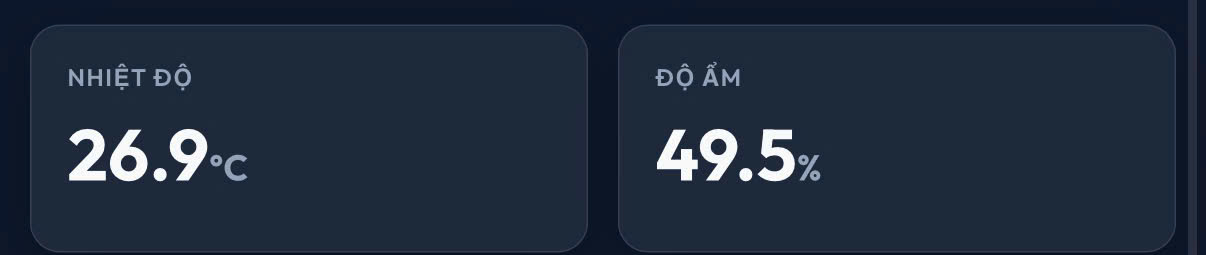
\includegraphics[width=0.55\textwidth]{pictures/task4_main_dashboard.png}
    \caption{Khối hiển thị tức thời trên giao diện chính của Web Server}
\end{figure}

Bên cạnh phần số liệu tức thời, giao diện còn tích hợp biểu đồ thời gian thực để mô tả sự thay đổi của nhiệt độ và độ ẩm theo thời gian. Nhờ đó, người dùng không chỉ biết giá trị hiện tại mà còn theo dõi được xu hướng tăng giảm của dữ liệu cảm biến trong một khoảng thời gian ngắn.

\begin{figure}[H]
    \centering
    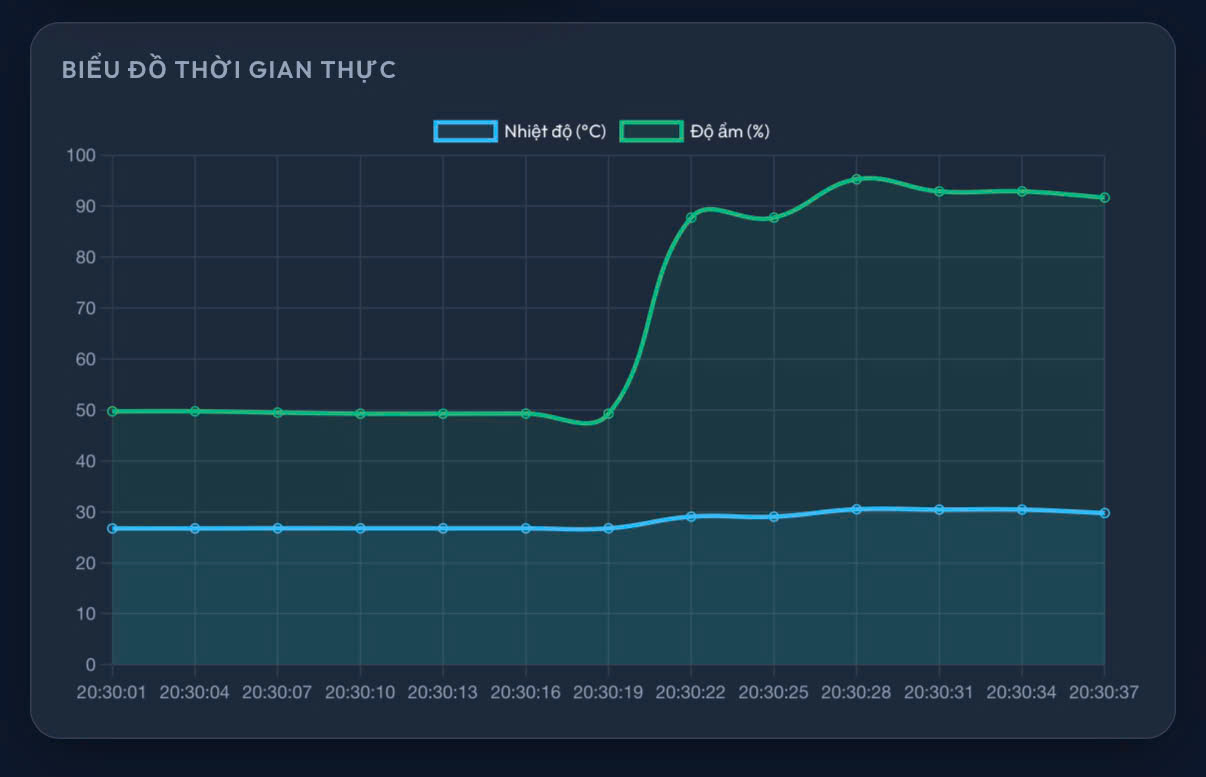
\includegraphics[width=0.8\textwidth]{pictures/task4_realtime_chart.png}
    \caption{Biểu đồ thời gian thực của nhiệt độ và độ ẩm trên giao diện Web Server}
\end{figure}

Sự kết hợp giữa phần số liệu tức thời, biểu đồ lịch sử ngắn hạn và các nút điều khiển giúp trang chính thực hiện tốt ba vai trò cùng lúc: giám sát nhanh, quan sát xu hướng và phát lệnh tới thiết bị. Đây là điểm thiết kế quan trọng giúp Web Server không chỉ là giao diện cấu hình mà còn là một bảng điều khiển cục bộ đúng với yêu cầu của Task 4.

\subsubsection{Trang cấu hình và quy trình kết nối Wi-Fi}
Hệ thống tách riêng phần cấu hình mạng thành một trang độc lập để người dùng mới có thể thao tác dễ dàng hơn. Tại đây, người dùng có thể chọn mạng Wi-Fi, nhập SSID ẩn nếu cần, điền mật khẩu và lưu cấu hình để thiết bị chuyển từ chế độ Access Point sang Station.

\begin{figure}[H]
    \centering
    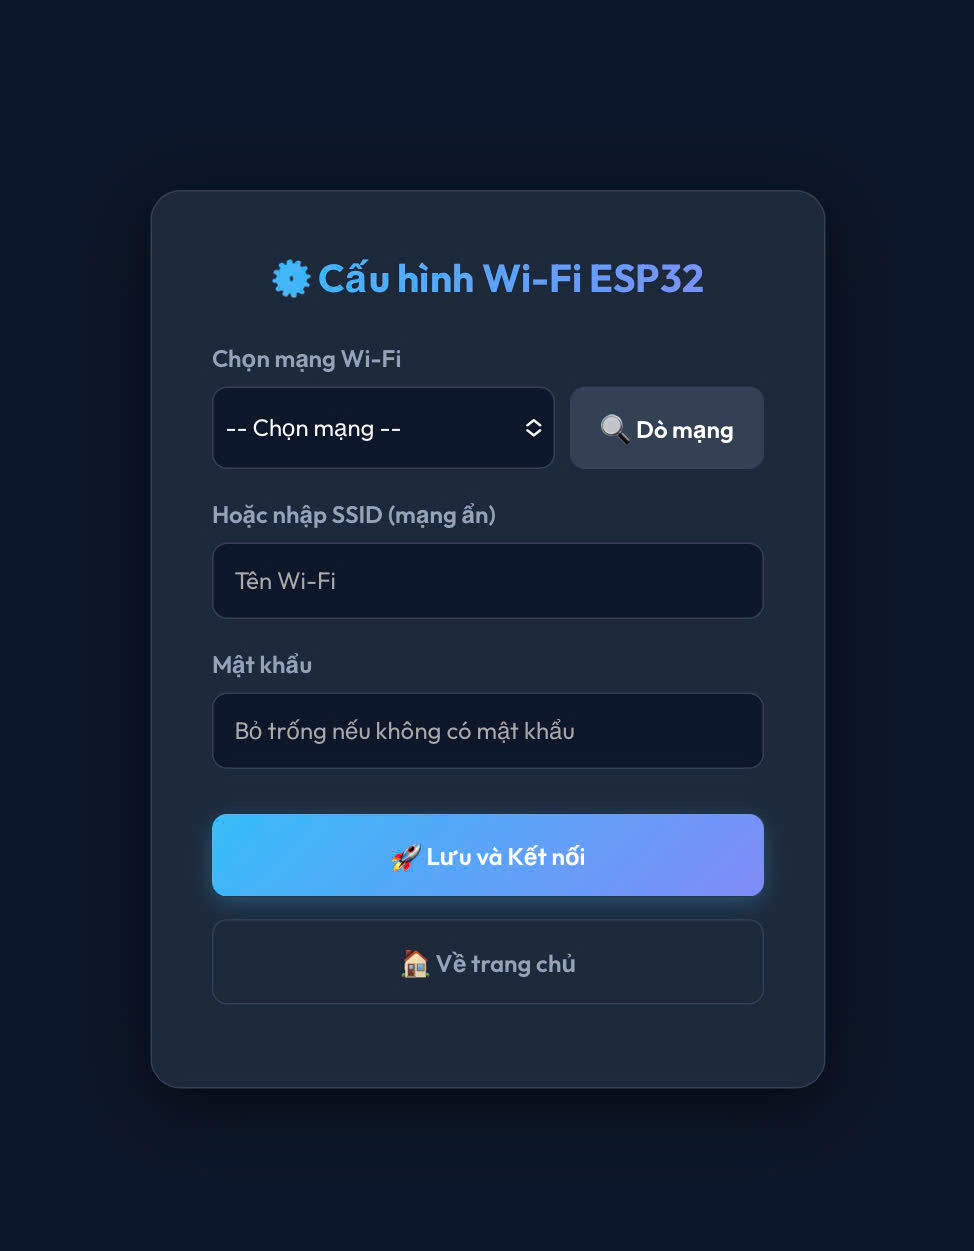
\includegraphics[width=0.42\textwidth]{pictures/task4_wifi_settings.png}
    \caption{Trang cấu hình Wi-Fi của Web Server}
\end{figure}

Sau bước nhập thông tin kết nối, hệ thống hỗ trợ quét danh sách các mạng khả dụng cùng cường độ tín hiệu. Chi tiết này rất hữu ích trong môi trường có nhiều mạng Wi-Fi hoạt động đồng thời, vì nó giúp người dùng chọn đúng điểm truy cập và đánh giá sơ bộ chất lượng tín hiệu trước khi lưu cấu hình.

\begin{figure}[H]
    \centering
    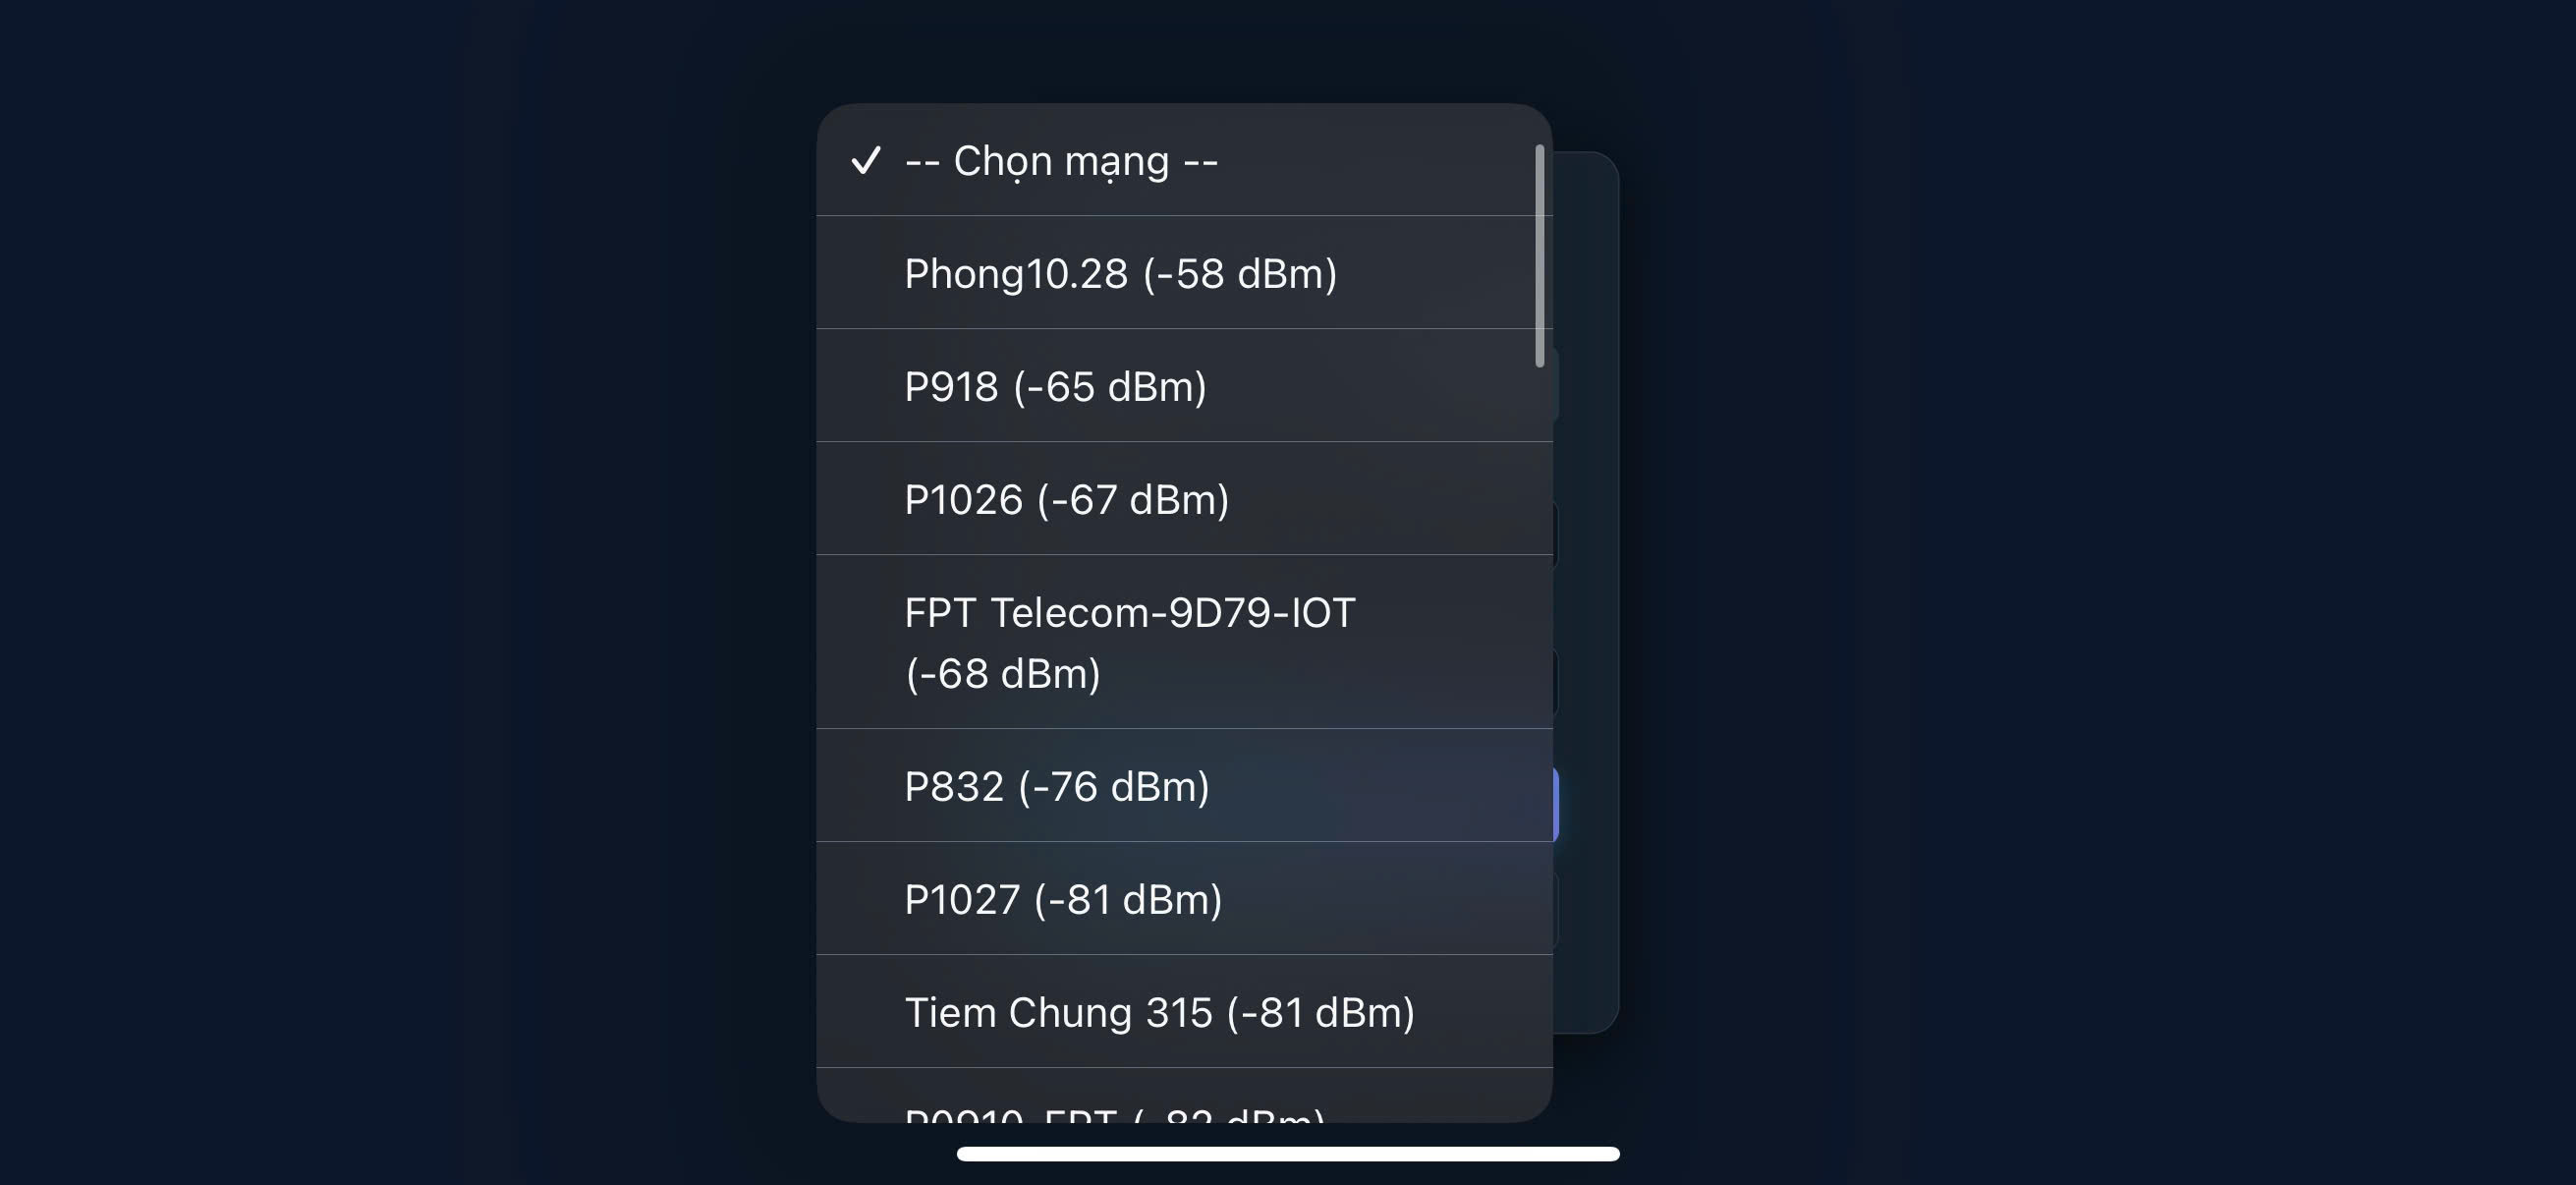
\includegraphics[width=0.82\textwidth]{pictures/task4_wifi_scan.png}
    \caption{Danh sách mạng Wi-Fi quét được và cường độ tín hiệu tương ứng}
\end{figure}

Hai hình trên thể hiện rõ quy trình cấu hình của hệ thống: trước tiên là nhập hoặc chọn thông tin mạng, sau đó là đối chiếu danh sách mạng quét được để hoàn tất kết nối. Cách tổ chức này làm giảm sai sót khi cấu hình và nâng cao trải nghiệm người dùng trong giai đoạn cài đặt ban đầu.

\subsubsection{Cơ chế Access Point và khôi phục cấu hình}
Một điểm đáng chú ý trong thiết kế là sự hiện diện của chân \texttt{BOOT\_PIN = 0}. Trong bối cảnh hệ thống nhúng, đây là tín hiệu phù hợp để triển khai cơ chế đưa thiết bị trở lại trạng thái cấu hình ban đầu hoặc cưỡng bức vào chế độ Access Point khi cần bảo trì. Nhờ cơ chế này, hệ thống không bị phụ thuộc tuyệt đối vào mạng Wi-Fi đã lưu trước đó; người dùng vẫn có thể phục hồi thiết bị ngay cả khi thay đổi router, quên mật khẩu hoặc xảy ra lỗi cấu hình.

Luồng vận hành tổng quát của Task 4 có thể mô tả như sau:
\begin{enumerate}
    \item Thiết bị khởi động và kiểm tra trạng thái cấu hình mạng.
    \item Nếu chưa có cấu hình hợp lệ, ESP32 phát Access Point và khởi tạo Web Server cục bộ.
    \item Người dùng truy cập giao diện web, nhập thông tin mạng tại \textit{Settings Page}.
    \item Hệ thống gọi \texttt{connectToWiFi()} để chuyển sang chế độ Station và tham gia mạng thật.
    \item Sau khi kết nối thành công, giao diện điều khiển tiếp tục được duy trì để thao tác với các thiết bị ngoại vi.
\end{enumerate}

\subsubsection{Đánh giá giải pháp}
Giải pháp Web Server ở chế độ Access Point mang lại nhiều ưu điểm thực tiễn cho hệ thống IoT. Thứ nhất, quá trình cấu hình ban đầu trở nên độc lập với hạ tầng mạng sẵn có, rất phù hợp trong các bài toán triển khai ngoài hiện trường. Thứ hai, việc đóng gói toàn bộ xử lý mạng trong một tác vụ riêng giúp tăng tính mô-đun và giảm nguy cơ ảnh hưởng tới các tác vụ thời gian thực khác. Cuối cùng, cách sắp xếp giao diện thành từng thành phần rõ ràng giúp người dùng dễ làm quen và giúp báo cáo thể hiện đúng ý tưởng thiết kế của Task 4.